\documentclass[journal,12pt,twocolumn]{IEEEtran}
\usepackage{graphicx}
\graphicspath{{./figs/}}{}
\usepackage{amsmath,amssymb,amsfonts,amsthm}
\newcommand{\myvec}[1]{\ensuremath{\begin{pmatrix}#1\end{pmatrix}}}
\usepackage{listings}
\usepackage{watermark}
\usepackage{titlesec}
\let\vec\mathbf
\lstset{
frame=single, 
breaklines=true,
columns=fullflexible
}
\thiswatermark{\centering \put(0,-105.0){
\includegraphics[scale=0.2]{iith.png}} }

\title{\mytitle}
\title{
Matrix Assignment - Lines
}
\author{Surajit Sarkar}
\begin{document}
\maketitle
\tableofcontents
\bigskip


\section{\textbf{Problem}}
One side of a rectangle lies along the line 4x+7y+5=0.
Two of its vertices are (-3,1) and (1,1).Find the equation of the other sides.


\section{\textbf{Solution}}
The direction of given line
\begin{equation}
    4\vec x+7 \vec y +5=0
\end{equation}
\begin{equation}
    7\vec y=-4\vec x-5
\end{equation}
\begin{equation}
    \vec y=\frac{-4}{7} \vec x-\frac{5}{7}
\end{equation}
\\
\begin{equation}
	\vec L =m= \myvec{1\\{\frac{-4}{7}}}
\end{equation}
The direction vector of line AC 
\begin{equation}
    d_{AC}=A-C=\myvec{-4\\0}
\end{equation}
AC is diagonal of the given rectangle between AC and AB
\\

where
\\
\begin{equation}
    \vec{Cos\theta} = {\frac{m^Td_{AC}}{\|m\|\|m_{AC}\|}}
\end{equation}
Vertices for A and B
\begin{equation}
	B-A=R_{\theta}{\myvec{C-A}} {\frac{\myvec{A-C}cos \theta}{\|A-C\|}}
\end{equation}
\begin{equation}
    D-A=R_{\frac{\pi}{2}-0} \myvec{C-A} sin\theta
\end{equation}
where
\begin{equation}
    R=\myvec{cos\theta&-sin\theta\\sin\theta&cos\theta}
\end{equation}
\\
Using python we get the point of B and D
\begin{lstlisting}
https://github.com/sssurajit/fwc/blob/main/line/codes/sline.py
\end{lstlisting}

\section{\textbf{Figure}}
\begin{figure}[h]
    \centering
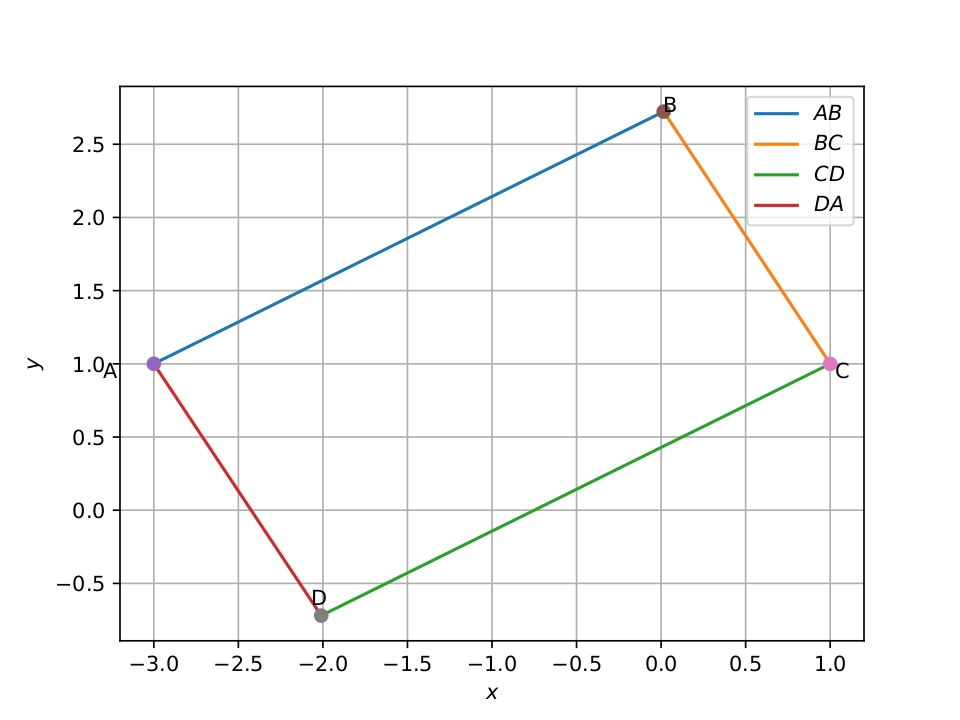
\includegraphics[width=\columnwidth]{fig.jpg}
    \label{fig:my_label}
\end{figure}


\section{\textbf{Code Link}}

\begin{lstlisting}
https://github.com/sssurajit/fwc/blob/main/line/codes/line.py
\end{lstlisting}
Execute the code by using the command\\
\textbf{python3 line.py}



\end{document}

